\documentclass[tikz,border=7pt]{standalone}
\usepackage{amsmath}
\usetikzlibrary{arrows.meta,positioning,fit}

\tikzset{
  comp/.style={draw,rectangle,minimum width=27mm,minimum height=12mm,align=center},
  test/.style={draw,rectangle,rounded corners=2pt,minimum width=29mm,minimum height=12mm,align=center},
  signal/.style={-{Latex[length=2.2mm]},thick}
}

\begin{document}
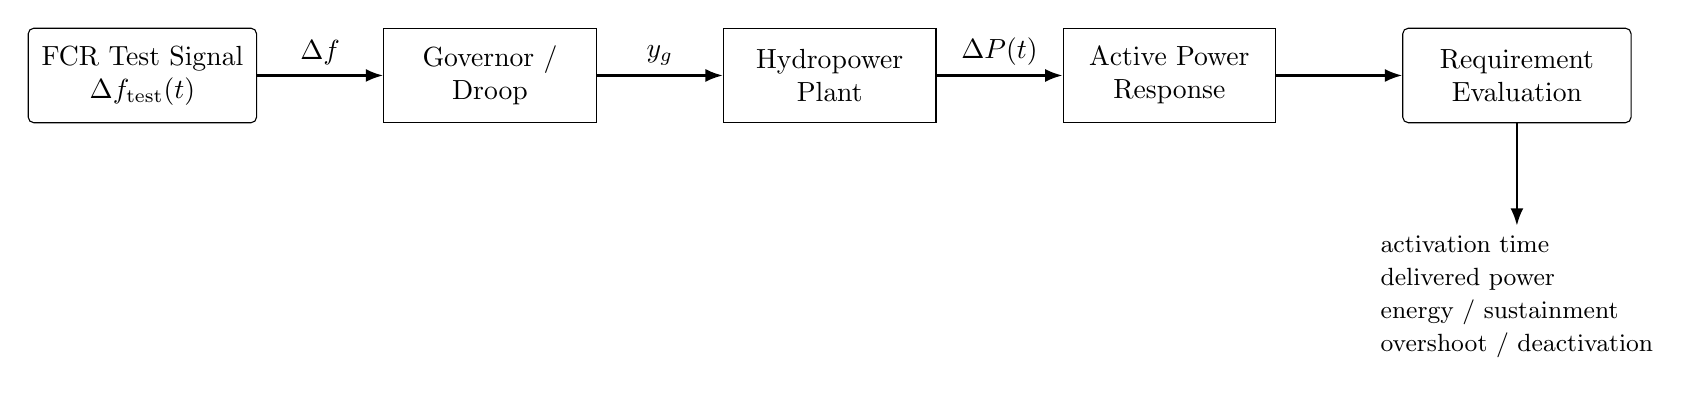
\begin{tikzpicture}[node distance=13mm and 16mm]

\node[test] (freq) {FCR Test Signal\\$\Delta f_{\mathrm{test}}(t)$};
\node[comp,right=of freq] (gov) {Governor /\\Droop};
\node[comp,right=of gov] (plant) {Hydropower\\Plant};
\node[comp,right=of plant] (power) {Active Power\\Response};
\node[test,right=of power] (eval) {Requirement\\Evaluation};

\draw[signal] (freq) -- node[above] {$\Delta f$} (gov);
\draw[signal] (gov) -- node[above] {$y_g$} (plant);
\draw[signal] (plant) -- node[above] {$\Delta P(t)$} (power);
\draw[signal] (power) -- (eval);

\node[below=13mm of eval,align=left] (metrics) {
\small activation time\\
\small delivered power\\
\small energy / sustainment\\
\small overshoot / deactivation
};

\draw[signal] (eval) -- (metrics);

\end{tikzpicture}
\end{document}
